\chapter{Diabetes mellitus}

Diabetes mellitus je chronické metabolické onemocnění. Vyznačuje se zvýšenou hladinou cukru v krvi, která se nazývá hyperglykémie. V normálu je hladina glykémie (koncentrace glukózy v krvi) mezi 3,8 a 5,6 mmol/l. Po jídle může glykémie stoupnout, neměla by však přesáhnout 7,8 mmol/l. O diabetes se jedná pokud jsou hodnoty vyšší než 11,1 mmol/l.

Hyperglykémie vzniká z nedostatku inzulinu nebo rezistencí buněk vůči jeho působení. Inzulin je hormon, který se tvoří v beta buňkách Langerhansových ostrůvků ve tkáni slinivky břišní. Tento hormon slouží k transportu glukózy z krve do tkáně, kde je využita k tvorbě energie nebo se zde ukládá ve formě glykogenu (v játrech) a tuků. Snižuje tak hladinu cukru v krevním řečišti. Pokud je hladina cukru nízká, produkce inzulinu se okamžitě zastaví  a hormony glukagon a adrenalin uvolní glukózu ze zásobních zdrojů pro zajištění fungování důležitých orgánů, především mozku, nervů a svalů.

Nedostatek inzulinu vede k nedostatečné utilizaci glukózy, která se hromadí v krvi. Dochází k poruše tvorby bílkovin, zvýšené tvorbě ketolátek, které se hromadí a způsobují překyselení organismu, a celkovému metabolickému rozvratu. Při hladině glykémie vyšší než 10-12 mmol/l začnou ledviny uvolňovat glukózu do moči spolu s dalšími látkami a vodou. To vše vyvolává dehydrataci, nevolnost, pokles krevního tlaku, poruchy vědomí.

Dlouhodobě přetrvávající hyperglykémie vede k poškození orgánů, především cév, nervového systému, ledvin a očí. Poškozením velkých cév může dojít k srdečnímu infarktu, mozkové příhodě nebo uzavření tepen v oblasti dolních končetin (ischemická choroba dolních končetin). U diabetických pacientů mají tato onemocnění komplikovanější průběh a vyšší úmrtnost. Nervové poškození je označováno jako diabetická neuropatie. Nejčastěji se objevuje v oblasti dolních končetin. končetina ztrácí citlivost, kůže vysychá a tvoří se defekt do kterého se snadno dostane infekce. Pokud není včas léčen, rozvíjí se syndrom diabetické nohy, který může vést k amputaci končetiny. poškození ledvin může vést k dialýze až k transplantaci ledvin. Poškození očí je příčinou vzniku šedého zákalu.

Bez léčby inzulinem může toto onemocnění vést k smrti. \cite{Diabetes.Psottova,Diabetes.TaiN} %Wikiskripta,cukrovka.cz


\section{Dělení diabetu}

Diabetes se dělí do čtyř základních skupin: diabetes 1. typu, diabetes 2. typu, gestační (těhotenský) diabetes, jiné specifické typy diabetu.

Diabetes mellitus 1. typu je autoimunitní onemocnění, kdy vlastní imunitní systém zničí beta buňky Langerhansových ostrůvků produkující inzulin. Langerhansových ostrůvků je ve slinivce kolem jednoho milionu a každý obsahuje zhruba 2000 beta buněk. Přesný počet se u každého liší. Při zničení 75-85 \% beta buněk nastává absolutní nedostatek inzulinu a objevují se zvýšené hodnoty glykémie.

Diabetes 1. typu se nejčastěji projeví již v dětském věku, ale může dlouho probíhat v latentní formě a projevit se až v pozdějším věku (LADA - latentní autoimunitní diabetes u dospělých). O diabetes se jedná pokud hodnota glykémie přesahuje 7 mmol/l nalačno. Po podání 75 g cukru pak glykémie přesahuje 11,1 mmol/l. Zda se jedná o diabetes 1. typu a ne diabetes 2. typu či jiné onemocnění způsobující vyšší hodnoty glykémie se určí stanovením hodnot glykovaného hemoglobinu a detekcí autoprotilátek, které vznikají při poškozování beta buněk. Příčina vzniku diabetu 1. typu není známá a proto není známa ani účinná prevence. Vlohy jsou často dědičné.

Nemoc se projevuje častým močením, které je v důsledku neschopnosti ledvin absorbovat přebytečnou glukózu. Z toho je pacient dehydratován, trpí žízní, nechutenstvím a celkovou slabostí. V důsledku hromadění ketolátek dochází k překyselení organismu, což může vést k poruchám vědomí. 

Diabetes mellitus 2. typu je metabolickou poruchou, kdy jsou buňky rezistentní vůči vlastnímu inzulinu, tj. buňky nejsou schopny vychytat inzulin v krevním oběhu, který by použili ke zpracování glukózy a úpravě hladiny glykémie. V počátcích beta buňky slinivky břišní reagují zvýšenou produkcí inzulinu (bezpříznaková inzulinová rezistence). Postupem času ale nejsou schopny dodávat potřebné množství inzulinu, nastává relativní nedostatek inzulinu a vzniká prediabetes a diabetes 2. typu. Příznaky jsou únava, žízeň, časté močení, pocit hladovění, hubnutí, infekce, špatné hojení a zhoršení zraku. Diabetes mellitus 2. typu vzniká v dospělosti na základě genetických předpokladů (inzulinová rezistence, nízká produkce inzulinu), rizikových faktorů a špatného životního stylu. Mezi ty patří nedostatek pohybu, nezdravá strava, nadváha a obezita (90 \% diabetiků 2. typu trpí nadváhou nebo je obézních), kouření, vysoká hladina cholesterolu a vysoký krevní tlak (hypertenze).

Gestační diabetes se objevuje v druhé polovině těhotenství a končí po porodu. Postihuje 17 \% těhotných žen, které k ní mají vrozenou dispozici. Neléčený diabetes má negativní dopad na vývoj plodu, který se musí vyrovnat se zvýšeným přísunem glukózy. Plod, který má produkci inzulinu v pořádku, pak výrazně rychleji roste. To může vést k předčasnému porodu, vrozeným vývojovým vadám, dechovým obtížím, poruchám srdečního rytmu, poruchám vývoje mozku, sklon k obezitě a rozvoje diabetu 2. typu.

Jiné specifické typy diabetu se označují jako sekundární diabetes, protože k rozvoji diabetu dochází v důsledku jiného onemocnění (např. zánět slinivky břišní) nebo v důsledku genetické poruchy (takzvané MODY).

V České republice je evidováno více než 900 000 pacientů s diabetem, kdy 92 \% připadá na diabetes 2. typu, 7 \% na diabetes 1. typu. Ročně přibude 60 tisíc nových diabetických pacientů a 22 tisíc umírá. Náklady na léčbu jednoho pacienta jsou okolo 26 000 Kč za rok. Ročně se tak vydá na léčbu diabetu 23 miliard Kč. \cite{Diabetes.Psottova,Diabetes.TaiN} %cukrovka.cz

Celosvětově je Světovou zdravotnickou organizací evidováno více než 422 milionů lidí s diabetem \cite{WHO}.

V této práci se budu zabývat detekcí karbohydrátů a fyzické aktivity u pacientů s diabetem 1. typu.


\section{Léčba}

Diabetes mellitus 1. typu je onemocnění z nedostatečné produkce inzulinu slinivkou břišní a vždy se léčí podáváním inzulinu. Způsob léčby a množství podávaného inzulinu je rozebráno v kapitole \ref{ch:inzulin}, způsoby podání v kapitole \ref{ch:pumpa}. Další možností pro pacienty diabetu 1. typu je transplantace slinivky břišní nebo transplantace samotných Langerhansových ostrůvků.

Při léčbě inzulinem se musí dbát na to, aby nenastala hypoglykémie. Hypoglykémie je stav, kdy dochází k poklesu cukru v krvi pod 3,9 mmol/l. Příznaky jsou pocení, třes, bušení srdce, slabost. Při těžké hypoglykémii dochází k poruchám vědomí a je nutná pomoc jiné osoby. Může nastat i smrt. K hypoglykémii často dochází při podání příliš velké dávky inzulinu snahou regulovat hladinu glukózy co nejvíce k normálním hodnotám. Z toho důvodu by pacient měl mít u sebe menší množství rychlých cukrů pro doplnění při zpozorování prvních příznaků.

Zvýšené riziko těžké hypoglykémie je při poruše tvorby adrenalinu v nadledvinách. Adrenalin se uvolňuje při nízké hladině cukru v krvi a je zodpovědný za příznaky hypoglykémie. Pacient pak není schopen rozpoznat rozvíjející se hypoglykémii. Tato porucha se označuje jako syndrom porušeného vnímání hypoglykémie.

Diabetes mellitus 2. typu se nejprve léčí úpravou životosprávy a kombinací perorálně podávaných antidiabetik (léky zvyšující produkci inzulinu a/nebo citlivost buněk k inzulinu). Pokud se těmito prostředky nedaří regulovat hladina cukru v krvi, přidá se k podávaným antidiabetikám léčba inzulinem.

Společnými režimovými opatřeními pro oba typy diabetu je monitorace glukózy (viz kapitola \ref{ch:monitorace}), dieta a fyzická aktivita.

Glykemie je závislá na jídle, druhu a frekvenci stravy, proto patří dieta mezi základní opatření při léčbě cukrovky. Pacient by měl znát složení jídla, především množství zkonzumovaných sacharidů. Strava by měla být vyvážená a v pravidelných intervalech.

Pohyb je důležitý protože napomáhá účinnosti inzulinu. Při pohybu se také využije více glukózy na energii, je prevencí proti nadváze a obezitě a celkově prospívá organismu. Fyzická aktivita tak výrazně snižuje koncentraci glukózy v krvi. Ideální hodnota glykémie před fyzickou aktivitou je 6-7 mmol/l. Při nižších hodnotách hrozí riziko hypoglykémie. Naopak při hodnotách >15 mmol/l se postupuje jako při hyperglykémii.

Cílem léčby je udržení doporučených hodnot vybraných ukazatelů popsaných v tabulce \ref{tab:ukazatele}. V závorkách jsou uvedeny přijatelné hodnoty rizikových pacientů. Pakliže se pacientovi dlouhodobě daří udržovat tyto doporučené hodnoty, sníží riziko komplikací spojených s diabetem.
\cite{Diabetes.Psottova} %,cukrovka.cz

\begin{table}[H]
\caption{Doporučené hodnoty vybraných ukazatelů}
\label{tab:ukazatele}
\centering
\begin{tabular}{|c|c|}
\hline 
\textbf{Ukazatel} & \textbf{Doporu\v{c}ené hodnoty}\tabularnewline
\hline 
\hline 
glykovaný hemoglobin & pod 45 (60) mmol/l\\ \hline 
glykémie naměřená před jídlem & 4-6 (pod 8) mmol/l\\ \hline 
glykémie naměřená po jídlem & 5-7,5 (pod 9) mmol/l\\ \hline 
krevní tlak & pod 130/80 (pod 140/90) mmHg\\ \hline 
celkový cholesterol & pod 4,5 mmol/l\\ \hline 
LDL-cholesterol & pod 2,5 mmol/l\\ \hline 
HDL-cholesterol (muži/ženy) & nad 1/1,2 mmol/l\\ \hline 
Celková denní dávka inzulinu & pod 0,6 j./kg\\
\hline 
\end{tabular}
\textit{Zdroj: www.cukrovka.cz \citep{cukrovka.cz}}
\end{table}


\subsection{Inzulinové režimy}
\label{ch:inzulin}

Schéma léčby inzulinem se volí individuálně. Cílem je korigovat deficit inzulinu a co nejpřesněji simulovat fyziologickou sekreci inzulinu. Pro každého diabetického pacienta je toto jiné z důvodu vlastního metabolismu, životního stylu a aktivit.

Zpravidla dělíme dávkování inzulinu na bazální hladinu inzulinu a bolusy. Bazální hladina inzulinu zajišťuje správnou hladinu glykémie mezi 5-9 mmol/l během dne a v noci. Dávka podaného inzulinu musí být nastavena tak, aby nedošlo k hypoglykémii. Inzulin se podává buď v jedné dávce na noc, nebo ve dvou menších dávkách ráno a večer. Účinnost podání bazálního inzulinu v jedné dávce večer je vidět na obrázku \ref{fig:inzulin} modře. Používají se středně nebo dlouho působící inzuliny.

Bolus slouží k aktuálnímu snížení hladiny glykémie. Používá se rychle působící prandiální inzulin, který začíná působit v krátkém čase a vrchol působení je mezi 1-2 hodinami. Bolus inzulinu se aplikuje zpravidla před jídlem, nebo pokud se naměří zvýšená hladina glykémie. Podání bolusu je znázorněno na obrázku \ref{fig:inzulin} červeně. Odhad poklesu glykémie po podání jedné jednotky inzulinu se vypočte 83 děleno celkovou denní dávkou inzulinu. \cite{Diabetes.Rybka,Inzulinove.rezimy}

\begin{figure}[H]
\caption{Působení inzulinu}
\label{fig:inzulin}
\centering
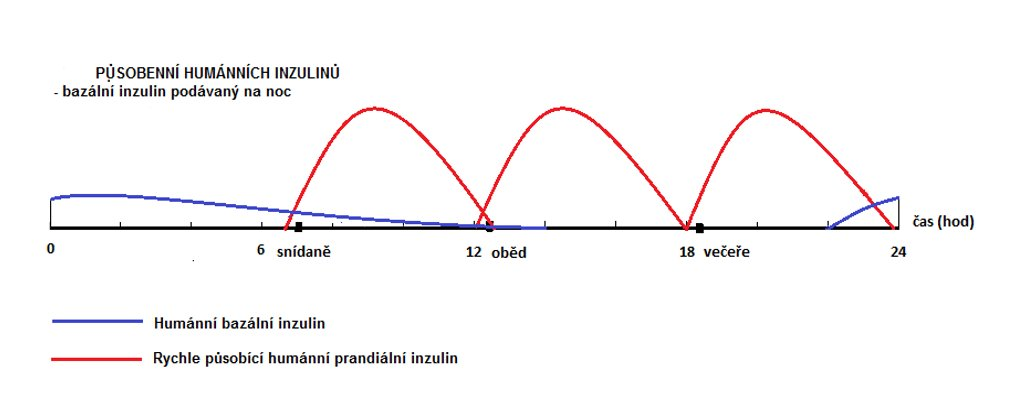
\includegraphics[width=1\textwidth]{img/diabetes/pusobeni-humannich-inzulinu.jpg}
\textit{Zdroj: www.cukrovka.cz \citep{cukrovka.cz}}
\end{figure}

Další možností je postupné dávkování inzulinu v malých dávkách během celého dne pomocí inzulinové pumpy (viz kapitola \ref{ch:pumpa}).


\subsection{Inzulinová pumpa}
\label{ch:pumpa}

Inzulin se podává injekčně do podkoží. Jednou z možností jsou inzulinová pera (aktuálně nejrozšířenější způsob podání inzulinu). Jedná se o lepší variantu klasické injekční stříkačky schopné dávkovat inzulin s přesností na 0,5 jednotky inzulinu.

Další možností aplikace inzulinu je inzulinová pumpa. Ta umožňuje kontinuální podání bazální dávky rychle působícího inzulinu. Simuluje tak reálnou funkci zdravé slinivky, která by za normálních okolností produkovala malé množství inzulinu pro udržení glykémie. Příjem jídla se vykryje nastavením požadovaného bolusu.

Na některých pumpách lze nastavit více bazálních dávek inzulinu přizpůsobených režimu daného dne (například víkendové aktivity nebo sport). Některé lze také propojit se systémem kontinuální monitorace glukózy, viz kapitola \ref{ch:monitorace}. \cite{Diabetes.Perusicova,Diabetes.Rybka} 

\subsection{Příjem karbohydrátů}

Karbohydráty (jiným názvem sacharidy či cukry) se po přijetí štěpí na glukózu, která je hlavním zdrojem energie pro lidské buňky. Při nedostatečném množství inzulinu nejsou buňky schopny glukózu zpracovat a ta se hromadí v krvi. Koncentrace glukózy v krvi se označuje jako glykémie.

Diabetický pacient musí hlídat množství přijatých karbohydrátů, které je nutné úměrně kompenzovat. Přijaté karbohydráty se projevují zvýšením koncentrace glukózy v krvi po dobu několika hodin (dle množství přijatých karbohydrátů). Pacient by měl rozdělit jídlo do šesti malých porcí v průběhu celého dne, z čehož 45 \% by měly být sacharidy. To spolu se správným dávkováním inzulinu pomáhá regulaci glykémie. Různé potraviny mají rozdílný glykemický index (jak rychle zvyšují hladinu glukózy v krvi). Je doporučena konzumace potravin s nízkým glykemickým indexem. Rychlé cukry s vysokým glykemickým indexem by se měly konzumovat v případě poklesu koncentrace glukózy v krvi (například příliš velká dávka inzulinu nebo fyzická aktivita).

Před jídlem se podává rychle působící prandiální inzulin, bolus. Inzulin se podává 30 minut před jídlem a vrchol působení je mezi 1-2 hodinami. Jeho množství by mělo odpovídat velikosti jídla. Pro výpočet množství karbohydrátů pokrytých 1 jednotkou inzulinu aplikovaného před jídlem vydělíme číslo 500 celkovou denní dávkou inzulinu. Pro výpočet bolusu pak vydělíme množství přijatých sacharidů vypočtenou hodnotou.

\subsection{Fyzická aktivita}

Během fyzické aktivity svalové buňky spotřebovávají glukózu a dochází tak k poklesu glykémie. Při fyzické zátěži je nutné častěji monitorovat hladinu glykémie, snížit množství dávkovaného inzulinu a případně podat sacharidy. Glykémie před cvičením by měla být mezi 6-7 mmol/l. Při nižších hodnotách je riziko hypoglykémie.

Hodnoty glykémie se měří před, během i po fyzické zátěži. Ideální je pro toto měření kontinuální monitorace glukózy (viz kapitola \ref{ch:cgms}). Měření glykémie po cvičení je důležité kvůli riziku vzniku takzvané pozdní hypoglykémie.

Před fyzickou zátěží je potřeba snížit množství podávaného inzulinu. V případě jednorázové aktivity se snižuje bolus inzulinu podávaný před jídlem o 20-50 \% dle náročnosti. Při dlouhodobější činnosti se snižuje množství bazálního inzulinu o 20-30 \%. Před a během zátěže je nutné pravidelně doplňovat sacharidy pro redukci rizika hypoglykémie.


\section{Monitorace glukózy}
\label{ch:monitorace}

Monitoring je důležitý pro správné určení léčby diabetologem.

Součástí monitorace je měření koncentrace glukózy a ketolátek v krvi a moči. Dále se kontroluje krevní tlak, hmotnost (BMI). Zaznamenávat by se měly denní dávky inzulinu, příjem karbohydrátů, hypoglykémie a hyperglykémie a situace vyžadující úpravu dávkování inzulinu, jako je zvýšená fyzická aktivita nebo nemoc. Při pravidelné kontrole u lékaře se vyšetřuje množství glykovaného hemoglobinu, cholesterolu, činnost ledvin a neuropatie.

Frekvence monitoringu je individuální a závislá na mnoha faktorech a potřebách daného pacienta. Selfmonitoring by se měl provádět denně před aplikací inzulinu, zhruba 3-4x denně, v noci v případě rizika hypoglykémie a v době nástupu dawn fenoménu (ranní hyperglykémie). Výsledek běžného denního měření se nazývá malý glykemický profil. Častější monitoring je třeba v případě zvláštních situací vyžadujících úpravu dávkování inzulinu a v těhotenství. Takové měření se nazývá malý glykemický profil.

Nejčastěji se glykémie měří glukometrem z kapky krve nanesené na diagnostický proužek. Tato metoda, která zahrnuje vpich do konečku prstu může být pro pacienta bolestivá a odradit ho od častějších měření. \cite{Diabetes.Pelikan}

\subsection{CGMS}
\label{ch:cgms}

Alternativou k jednorázovým měřením je kontinuální monitorace glukózy (CGMS - Continuous Glucose Monitoring System). Pro měření se zavede elektrochemický glukózový senzor do podkoží, kde se měří koncentrace glukózy v plazmě v intersticiální (mezibuněčné) tekutině. Tento systém umožňuje měření hladiny glukózy po celý den v minutových nebo pětiminutových intervalech (na českém trhu jsou dostupné přístroje měřící v pětiminutových intervalech). To umožňuje sledovat vývoj glykémie během dne a stanovit tak glykemický profil pacienta.

Hodnoty ze senzoru a hodnoty naměřené z krve se mohou lišit. Protože měření probíhá v intersticiální tekutině, kam se glukóza dostává z krve s menším zpožděním, jsou naměřené hodnoty také se zpožděním vůči reálné hodnotě v krvi. V některých případech jsou koncentrace v intersticiální tekutině nižší než v krvi, zejména v noci. Senzor se musí pro správnou funkci denně kalibrovat (alespoň 2x) hodnotami naměřenými z krve při stabilní glykémii. \citep{Diabetes.Perusicova}

Přístroje disponují alarmem signalizujícím vzestup či pokles glykémie. Do CGMS uživatel ručně zadává množství přijatých karbohydrátů z jídla a fyzická aktivita. Z dat CGMS pak lze lépe určit vývoj glykémie v závislosti na daných aktivitách.

Některé přístroje umožňují integraci s kompatibilní inzulinovou pumpou a zadání požadované bazální hladiny inzulinu a bolusů. Aktuální hybridní systémy jsou schopny upravovat hladinu bazálu podle naměřených hodnot. Inzulinová pumpa tak dávkuje potřebné množství inzulinu bez nutnosti častého zásahu pacienta. Takové systémy se někdy označují jako umělá slinivka. Příkladem je systém OpenAPS, který ale není oficiálně schválený jako zdravotnický prostředek a tudíž není zaručena jeho správná funkcionalita. Dalším příkladem aplikace pro řízení inzulinové pumpy na základě dat CGMS je SmartCGMS, který je vyvíjen na katedře Informatiky a výpočetní techniky na ZČU (viz kapitola \ref{ch:smartcgms}). Plně autonomní systém zatím neexistuje z důvodu, že hladinu glukózy ovlivňuje mnoho faktorů, které přístroje na trhu nejsou schopny spolehlivě rozeznat. Jedná se především o rychlé zvýšení glykémie po jídle a podání odpovídajícího bolusu.

Rizikem autonomních systémů je podání příliš velkého množství inzulinu a stavu hypoglykémie, která je mnohonásobně horší než riziko hyperglykémie. Řešením by mohl být dávkovač glukagonu, který by při poklesu glykémie hladinu opět vyrovnal. %\citep{cukrovka.cz}